\begin{figure}[htbp]
\centering
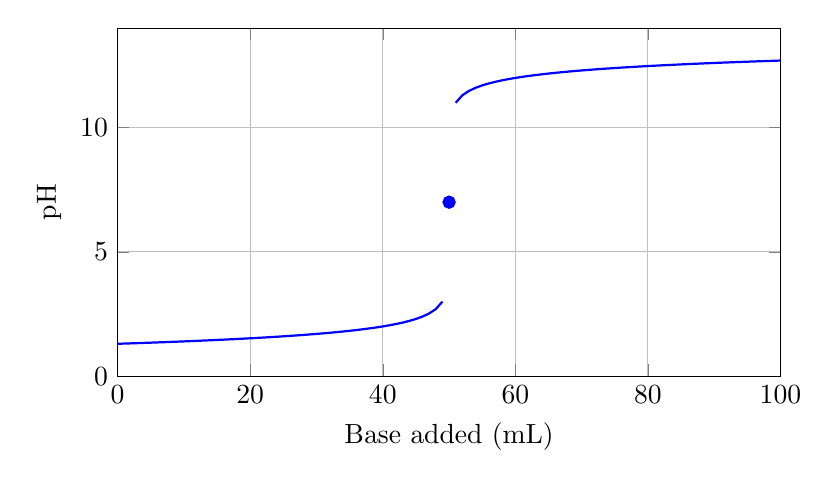
\begin{tikzpicture}
\begin{axis}[
    width=10cm, height=6cm,
    xlabel={Base added (mL)},
    ylabel={pH},
    xmin=0, xmax=100,
    ymin=0, ymax=14,
    grid=major
]
\addplot[blue, thick, domain=0:49, samples=50] {-log10(0.1*(50-x)/100)};
\addplot[blue, thick, domain=51:100, samples=50] {14 + log10(0.1*(x-50)/100)};
\addplot[blue, thick, mark=*] coordinates {(50,7)};
\end{axis}
\end{tikzpicture}
\caption{Typical pH titration curve showing high gain near equivalence.}
\label{fig:ph_titration}
\end{figure}
